\section{Corriente y resistencia}
  \subsection{Corriente eléctrica}
    \PN La cantidad de flujo de las cargas eléctricas depende del material a través del cual pasan las cargas y de la
    diferencia de potencial que existe de un extremo al otro del material. Siempre que hay un flujo neto de carga a
    través de alguna región, se dice que existe una corriente eléctrica.

    \PN Para definir la corriente con mayor precisión, suponga que las cargas tienen un movimiento perpendicular a una
    superficie A. La corriente es la proporción a la cual circula la carga a través de esta superficie. Si $Q$ es la
    cantidad de carga que pasa a través de esta superficie en un intervalo de tiempo $t$, la corriente promedio
    $I_{prom}$ es igual a la carga que pasa a través de A por unidad de tiempo:
    \begin{equation*}
      I_{prom} = \frac{\Delta Q}{\Delta t}
    \end{equation*}

    \PN Si la proporción a la que circula la carga varía en el tiempo, entonces, la corriente también varía en el
    tiempo; se define de la corriente instantánea $I$ como el límite diferencial de la corriente promedio:
    \begin{equation*}
      I \equiv \frac{dQ}{dt}
    \end{equation*}

    \PN La unidad del SI para la corriente es el \textbf{ampere} (A):
    \begin{equation*}
      1 \ \text{A} = 1 \ \frac{\text{C}}{\text{s}}
    \end{equation*}

    \PN Las partículas con carga que pasan a través de la superficie pueden ser positivas, negativas, o ambas. Es una
    regla convencional asignar a la corriente la misma dirección que la del flujo de la carga positiva. En los
    conductores eléctricos, como cobre o aluminio, la corriente está ocasionada por el movimiento de electrones con
    carga negativa. Por lo tanto, en cualquier conductor, la dirección de la corriente es la opuesta a la dirección del
    flujo de los electrones.

    \PN Es común referirse a una carga en movimiento (positiva o negativa) como un portador de carga móvil.

  \subsection{Resistencia}
    \PN Piense en un conductor de área de sección transversal A que transporta una corriente $I$. La densidad de
    corriente $J$ en el conductor se define como la corriente por unidad de área. La densidad de corriente es igual a
    \begin{equation*}
      J \equiv \frac{I}{A}
    \end{equation*}

    \PN donde $J$ tiene unidades en el SI de amperes por cada metro cuadrado. Esta expresión es válida sólo si la
    densidad de corriente es uniforme y sólo si la superficie del área de sección transversal A es perpendicular a la
    dirección de la corriente.

    \PN Tan pronto como se mantiene una diferencia de potencial a través del conductor se establece una densidad de
    corriente y un campo eléctrico. En algunos materiales, la densidad de corriente es proporcional al campo eléctrico:
    \begin{equation*}
      J = \sigma E
    \end{equation*}

    \PN donde la constante de proporcionalidad $\sigma$ se conoce como conductividad del conductor.

    \PN Los materiales que obedecen la ley de Ohm y por tanto cumplen esta simple correspondencia entre $E$ y $J$, se
    conocen como materiales \textit{óhmicos}. Sin embargo, se ha encontrado experimentalmente que no todos los
    materiales tienen esta propiedad.

    \PN Si consideramos un segmento de alambre recto de área de sección transversal uniforme Ay de longitud $l$,
    obtendrá una ecuación que resulte útil en aplicaciones prácticas. De un extremo al otro del alambre se mantiene una
    diferencia de potencial $\Delta V = V_{b} - V_{a}$, lo que genera en el alambre un campo eléctrico y una corriente.
    Si supone que el campo es uniforme, la diferencia de potencial está relacionada con el campo mediante la relación
    \begin{equation*}
      \Delta V = E l
    \end{equation*}

    \PN Por lo tanto, la densidad de corriente en el alambre se expresa en la forma
    \begin{equation*}
      J = \sigma E = \sigma \frac{\Delta V}{l}
    \end{equation*}

    \PN Ya que $J = I/A$, la diferencia de potencial a través del alambre es
    \begin{equation*}
      \Delta V = \frac{l}{\sigma} \ J = \left(\frac{l}{\sigma A}\right) \ I = RI
    \end{equation*}

    \PN La cantidad $R = l/\sigma A$ se conoce como la resistencia del conductor que es definida como la relación de la
    diferencia de potencial aplicada a un conductor entre la corriente que pasa por el mismo:
    \begin{equation*}
      R \equiv \frac{\Delta V}{I}
    \end{equation*}

    \PN Al estudiar los circuitos eléctricos utilizará esta ecuación una y otra vez. Con este resultado se observa que
    la resistencia tiene unidades del SI de volts por ampere. Un volt por ampere se define como un \textbf{ohm}
    ($\ohm$):
    \begin{equation*}
      1 \ \ohm = 1 \ \frac{\text{V}}{\text{A}}
    \end{equation*}

    \PN La mayoría de los circuitos eléctricos usan elementos llamados \textbf{resistores} para controlar la corriente
    en las diferentes partes del circuito.

    \PN El recíproco de la conductividad es la \textbf{resistividad} $\rho$:
    \begin{equation*}
      \rho = \frac{1}{\sigma}
    \end{equation*}

    \PN donde $rho$ está en ohms-metros ($\ohm m$). Ya que $R = l/\sigma A$, es posible expresar la resistencia a lo
    largo de la longitud de un bloque uniforme de material de la forma
    \begin{equation*}
      R = \rho \ \frac{l}{A}
    \end{equation*}

  \subsection{Resistencia y temperatura}
    \PN En un intervalo limitado de temperatura, la resistividad de un conductor varía prácticamente de manera lineal
    con la temperatura, de acuerdo con la expresión
    \begin{equation*}
      \rho = \rho_{0} \left[1 + \alpha (T - T_{0})\right]
    \end{equation*}

    \PN donde $\rho$ es la resistividad a cierta temperatura $T$ (en grados Celsius), $\rho_{0}$ la resistividad en
    alguna temperatura de referencia $T_{0}$ (por lo general 20ºC), y $\alpha$ el \textbf{coeficiente de temperatura de
    resistividad}. El coeficiente de temperatura de resistividad se expresa como
    \begin{equation*}
      \alpha = \frac{1}{\rho_{0}} \ \frac{\Delta \rho}{\Delta T}
    \end{equation*}

    \PN donde $\Delta \rho = \rho - \rho_{0}$ es el cambio en la resistividad durante el intervalo de temperatura
    $\Delta T = T - T_{0}$.

    \PN Ya que la resistencia es proporcional a la resistividad, la variación en la resistencia de una muestra es
    \begin{equation*}
      R = R_{0} \left[1 + \alpha (T - T_{0})\right]
    \end{equation*}

    \PN donde $R_{0}$ es la resistencia a la temperatura $T_{0}$.

  \VS
  \PN \textbf{\underline{Superconductores}}
  \PN Existe una clase de metales y de compuestos cuya resistencia disminuye hasta cero cuando llegan a una cierta
  temperatura $T_{c}$, conocida como temperatura crítica. Estos materiales se conocen como \textbf{superconductores}.

  \begin{figure}[H]
  \centering
    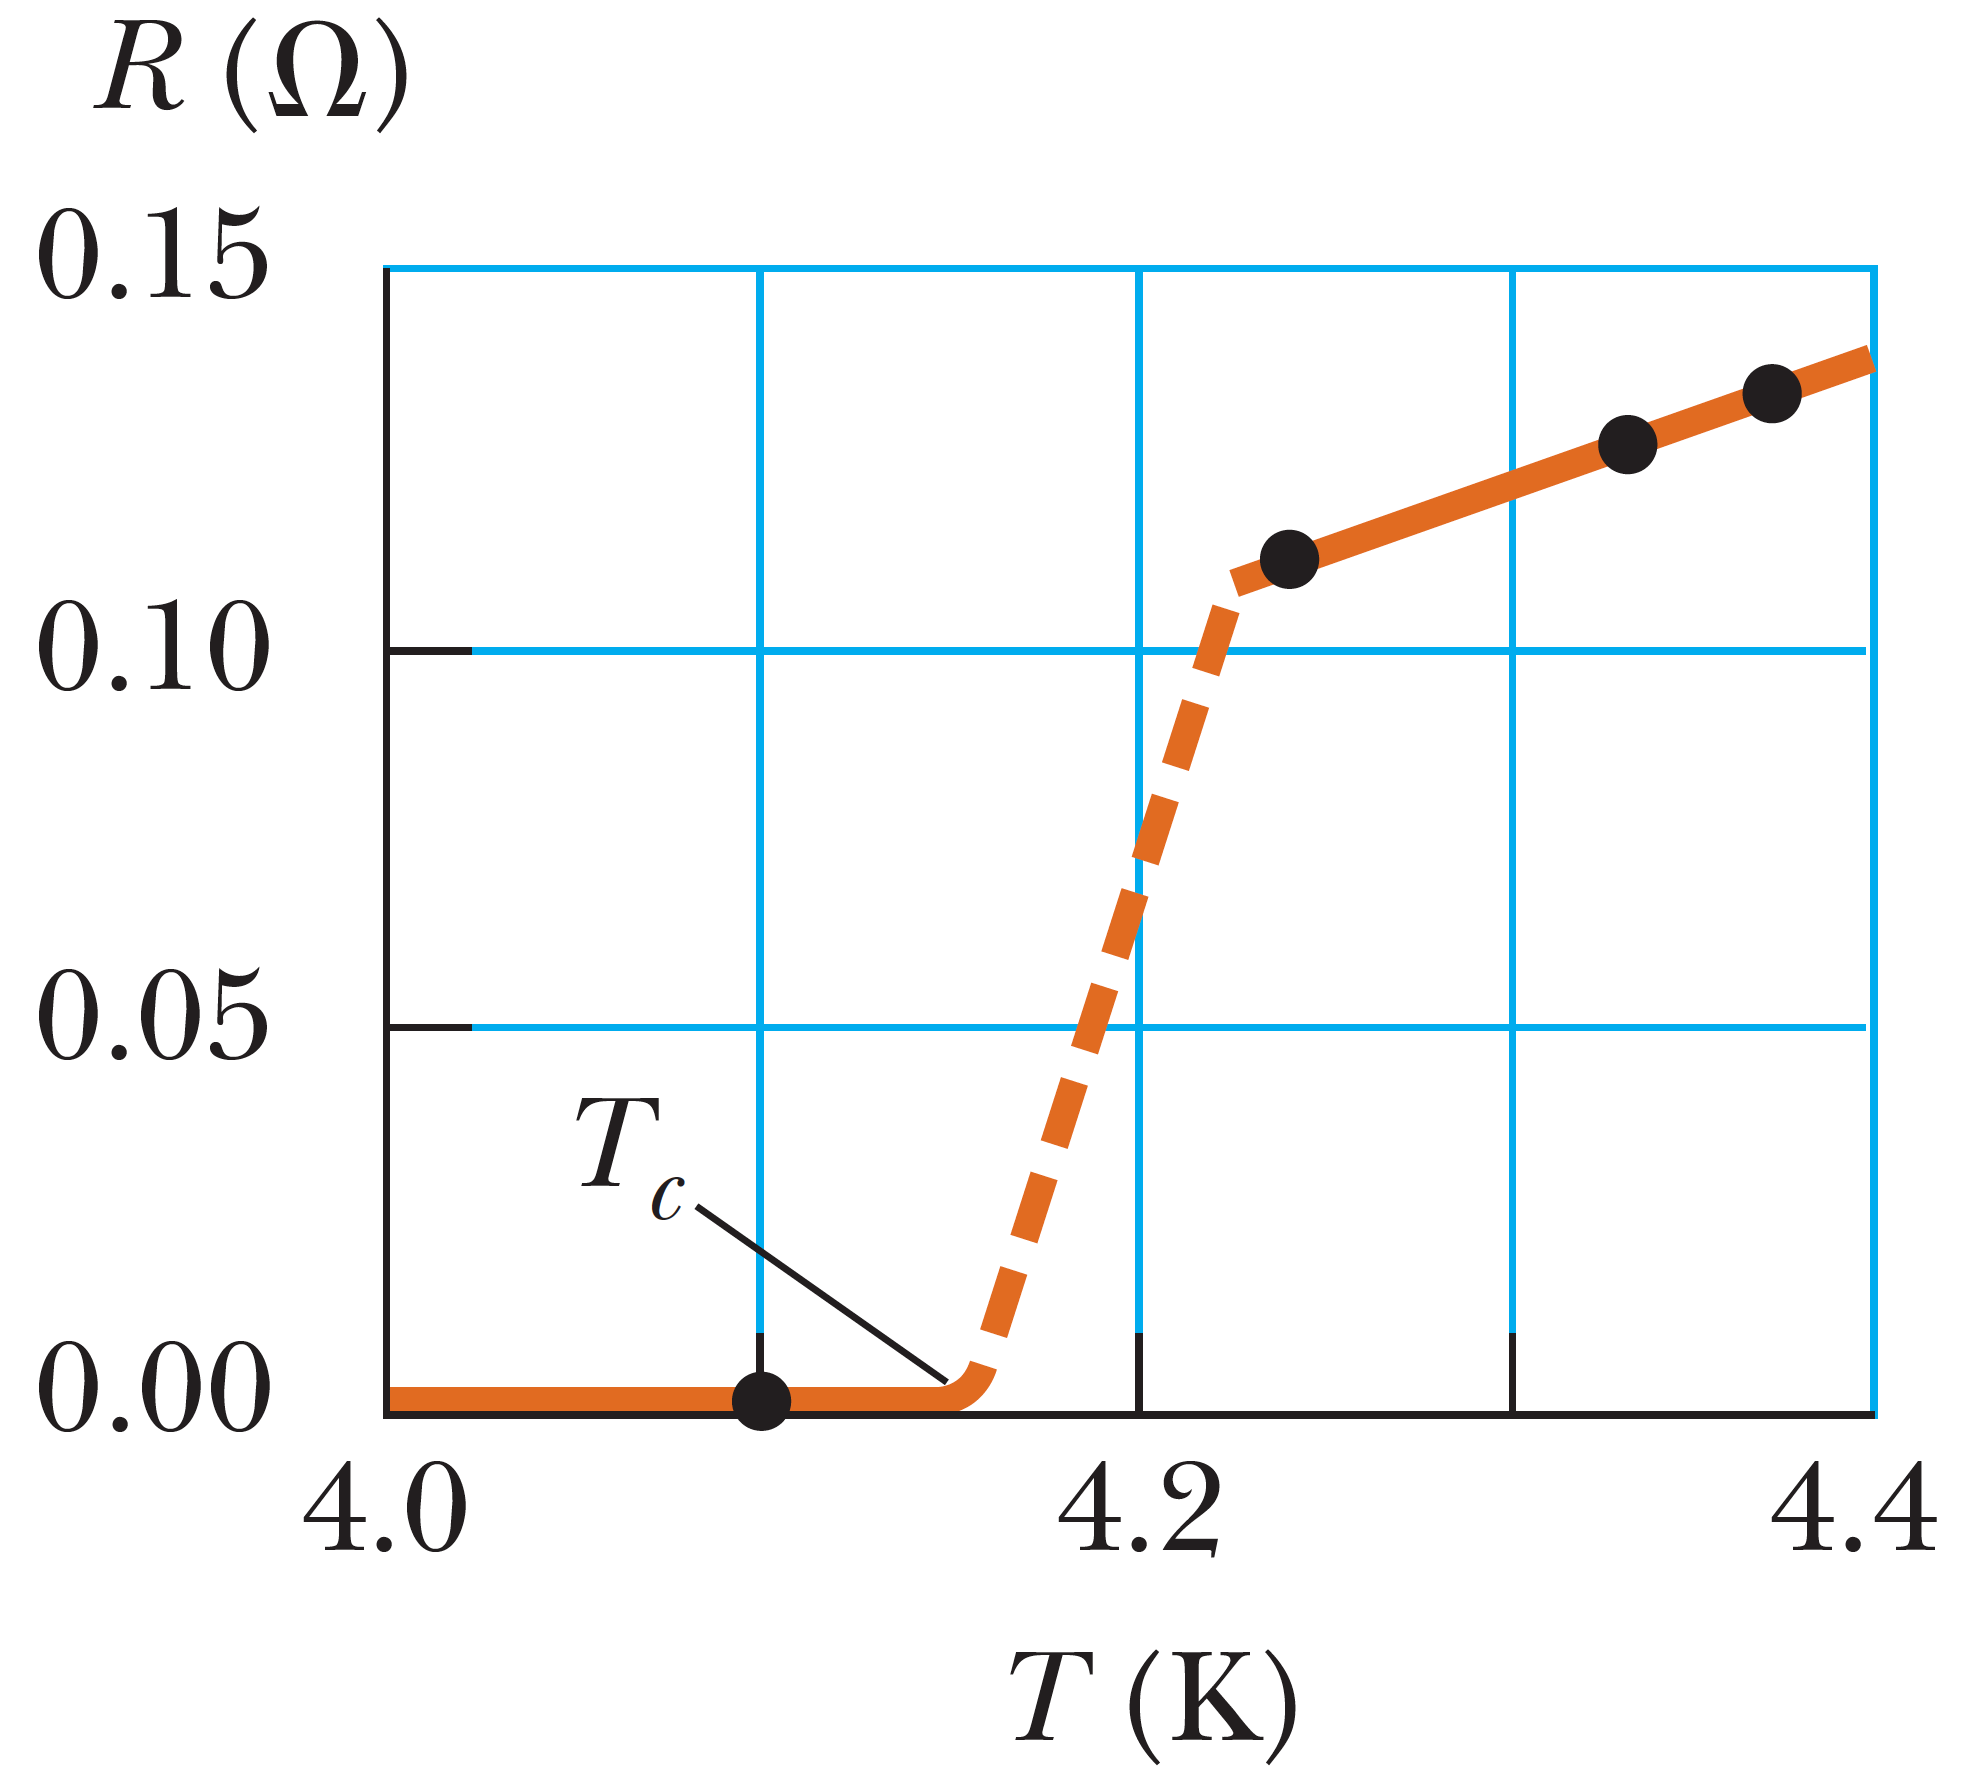
\includegraphics[width=0.35\textwidth]{4/figure_8}
    \caption{Resistencia en función de la temperatura para una muestra de mercurio (Hg).}
  \end{figure}

  \subsection{Potencia eléctrica}
    \PN En los circuitos eléctricos típicos, la energía se transfiere de una fuente, como una batería, a algún
    dispositivo, como sería una lámpara o un receptor de radio. Por ello conviene determinar una expresión que permita
    calcular la rapidez de transferencia de esta energía.

    \begin{figure}[H]
    \centering
      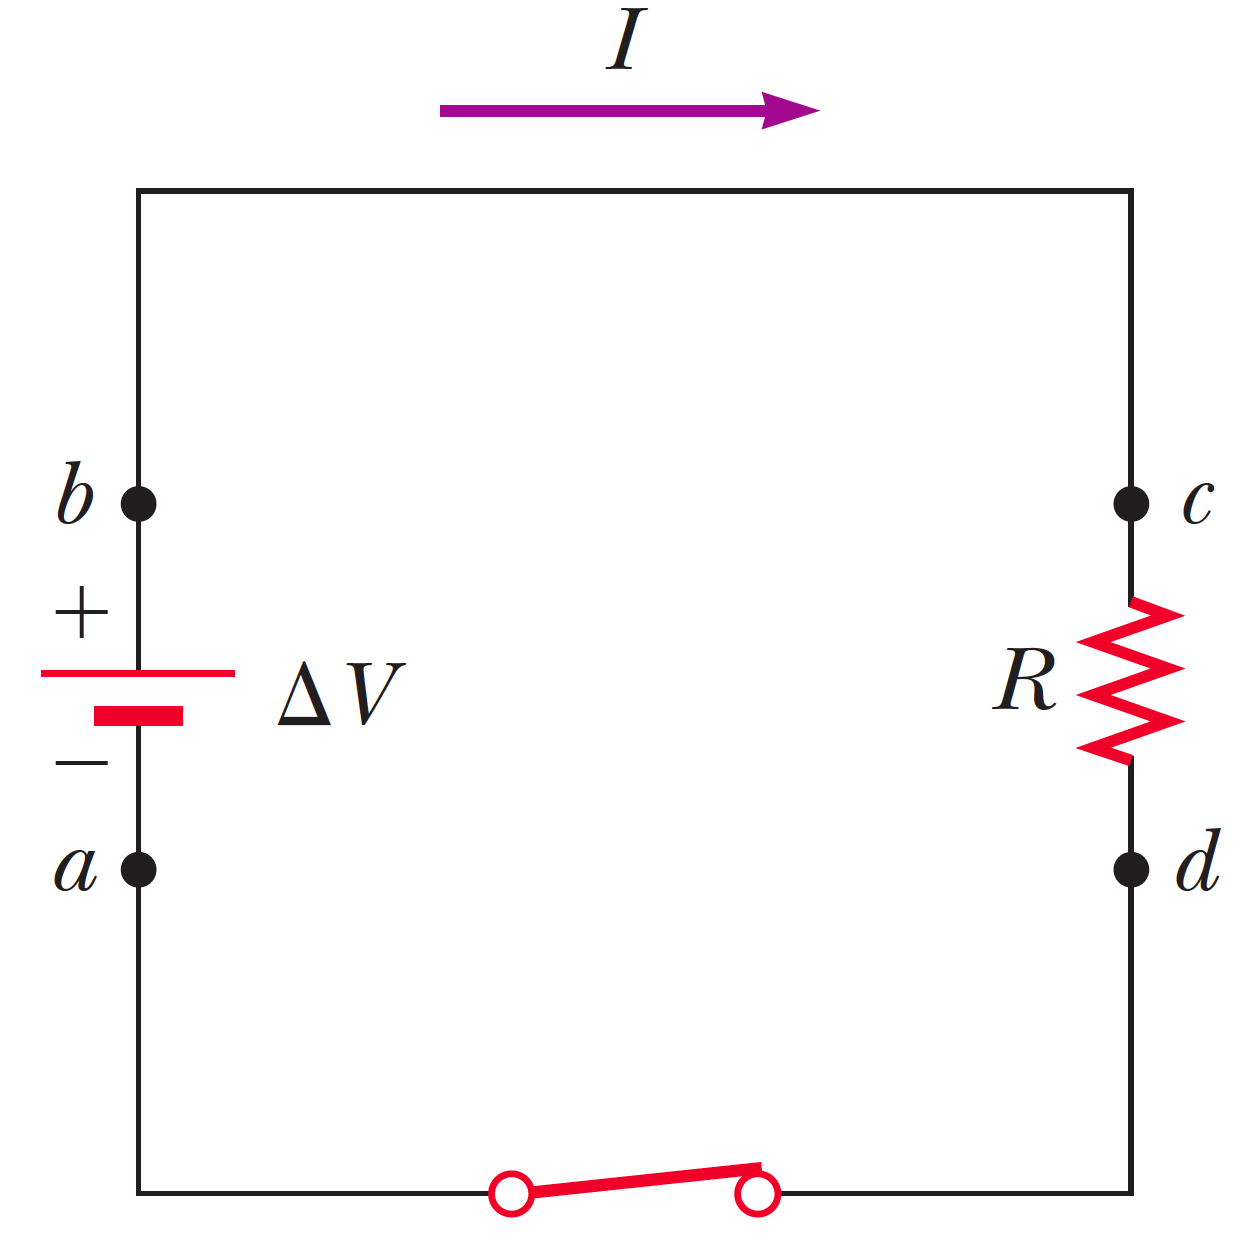
\includegraphics[width=0.25\textwidth]{4/figure_9}
      \caption{Circuito constituido por un resistor de resistencia $R$ y una batería con una diferencia de potencial
      $\Delta V$ entre sus terminales. La carga positiva fluye en dirección de las manecillas del reloj.}
    \end{figure}

    \PN Considere ahora la rapidez a la cual el sistema pierde energía potencial eléctrica conforme la carga $Q$ pasa a
    través del resistor:
    \begin{equation*}
      \frac{dU}{dt} = \frac{d}{dt} \ (Q \ \Delta V) = \frac{dQ}{dt} \ \Delta V = I \ \Delta V
    \end{equation*}

    \PN donde $I$ es la corriente en el circuito. El sistema recupera su energía potencial cuando la carga pasa a través
    de la batería, a expensas de la energía química de la misma. La rapidez a la cual el sistema pierde energía
    potencial conforme la carga pasa a través del resistor es igual a la rapidez a la cual el sistema adquiere energía
    interna en el resistor. Por lo tanto, la potencia $\mathcal{P}$ que representa la rapidez a la cual se entrega
    energía al resistor, es
    \begin{equation*}
      \mathcal{P} = I \ \Delta V
    \end{equation*}

    \PN Se deduce este resultado si considera una batería que entrega energía a un resistor. Para calcular la potencia
    entregada por una fuente de voltaje a cualquier dispositivo que tenga una corriente $I$ y esté sujeto a una
    diferencia de potencial $\Delta V$ entre sus terminales. Apartir de que un resistor $\Delta V = IR$, la potencia
    entregada al resistor tiene una expresión alterna
    \begin{equation*}
      \mathcal{P} = I^{2} R = \frac{(\Delta V)^{2}}{R}
    \end{equation*}

    \PN Cuando $I$ se expresa en amperes, $\Delta V$ en volts y $R$ en ohms, la unidad del SI para la potencia es el
    \textbf{watt}. El proceso mediante el que se pierde potencia en forma de energía interna en un conductor de
    resistencia $R$, a menudo se llama \textit{calentamiento joule}.
